\section{Auswertung}
\label{sec:Auswertung}
\subsection{Überprüfung der Braggbedingung}
Zur Überprüfung der Braggbedingung wurde der Kristallwinkel auf $\SI{14}{\degree}$ eingestellt.
Die Messdaten befinden sich in Tabelle \ref{tab:bragg}.

\begin{table}
  \centering
  \caption{Messwerte zur Überprüfung der Braggbedingung.}
  \label{tab:bragg}
  \begin{tabular}[t]{c@{} S[table-format=2.1] S[table-format=3.0]}
   \toprule
     {$2\, \theta \, / \, \si{\degree}\:\:$} & {$\text{Rate} \, /  \, \si{\per\second}$} \\\midrule
     \csvreader[no head,
     late after line=\\,
     late after last line=\\\bottomrule,
     filter test={\ifnumless{\thecsvinputline}{22}}]%
     {data/braggbedingung.csv}{}%
     {$\SI{\csvcoli}{}$ & $\SI{\csvcolii}{}$}%
   \end{tabular}
   \begin{tabular}[t]{c@{} S[table-format=2.1] S[table-format=3.0]}
    \toprule
      {$2\, \theta \, / \, \si{\degree}\:\:$} & {$\text{Rate} \, /  \, \si{\per\second}$} \\\midrule
     \csvreader[filter test={\ifnumgreater{\thecsvinputline}{21}},
     late after line=\\,
     late after last line=\\\bottomrule]%
     {data/braggbedingung.csv}{}%
    {$\SI{\csvcoli}{}$ & $\SI{\csvcolii}{}$}%
  \end{tabular}
\end{table}
\begin{figure}
  \centering
  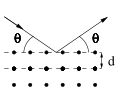
\includegraphics{bragg.pdf}
  \caption{Plot zur Überprüfung der Bragg-Bedingung.}
  \label{fig:bragg}
\end{figure}

Das Maximum der Intensität lässt sich aus dem Plot zu $\SI{13.9}{\degree}$ bestimmen und weicht um $\SI{0.7}{\percent}$ vom eingestellten Winkel ab.

\FloatBarrier
\subsection{Das Emissionsspektrum einer Cu-Röntgenröhre}

Die gemessenen Winkel und die entsprechenden Counts pro Sekunde sind in der Tabelle \ref{tab:Emissionsspektrum} zusammengefasst.
Diese wurden graphisch in Abbildung \ref{fig:Emissionsspektrum} dargestellt.
Dort können die K$_\alpha$ und K$_\beta$ abgelesen werden.

\begin{figure}
  \centering
  \includegraphics{build/emission.pdf}
  \caption{Graphische Darstellung der Messergebnisse und kenntlich machen der K$_\alpha$- und K$_\beta$-Linien und des Bremsberges.}
  \label{fig:Emissionsspektrum}
\end{figure}

\begin{table}
  \centering
  \caption{Die zu den entsprechenden Winkeln gemessenen Counts.}
  \label{tab:Emissionsspektrum}
  \begin{tabular}[t]{c|c}
    \toprule
      $2 \cdot \theta \, / \, \si{\degree}$ & $\text{Counts} \, / \, \si{\per\second}$ \\
      \midrule
      \csvreader[no head,
      late after line=\\,
      late after last line=\\\bottomrule,
      filter test={\ifnumless{\thecsvinputline}{38}}]%
      {data/emissionsspektrum.csv}{}%
      {\csvcoli & \csvcolii }%
  \end{tabular}
  \begin{tabular}[t]{c|c}
    \toprule
      $2 \cdot \theta \, / \, \si{\degree}$ & $\text{Counts} \, / \, \si{\per\second}$ \\
      \midrule
      \csvreader[filter expr={ test{\ifnumgreater{\thecsvinputline}{37}}
                           and test{\ifnumless{\thecsvinputline}{75}}},
      late after line=\\,
      late after last line=\\\bottomrule]%
      {data/emissionsspektrum.csv}{}%
      {\csvcoli & \csvcolii}%
  \end{tabular}
  \begin{tabular}[t]{c|c}
    \toprule
      $2 \cdot \theta \, / \, \si{\degree}$ & $\text{Counts} \, / \, \si{\per\second}$ \\
      \midrule
      \csvreader[filter test={\ifnumgreater{\thecsvinputline}{74}},
      late after line=\\,
      late after last line=\\\bottomrule]%
      {data/emissionsspektrum.csv}{}%
      {\csvcoli & \csvcolii}%
  \end{tabular}
\end{table}

Der Grenzwinkel wird aus den Messdaten zu $\theta = \SI{5.0}{\degree}$ bestimmt.
Aus der Braggbedingung \eqref{eqn:bragg} ergibt sich somit für die Wellenlänge bei einer Gitterkonstante des LiF-Kristalls von $\SI{201.4}{\pico\metre}$:

\begin{align*}
  \lambda_\text{Grenz} = \SI{35.11}{\pico\metre}
\end{align*}

Die maximale Energie des Bremsspektrums wird dann mittels der Gleichung \eqref{eqn:Energie} bestimmt.
Dies wird mit dem theoretischen wert für E$_\text{kin, max} = e_0 U$ verglichen.
Es ergibt sich dann:

\begin{align*}
  \text{E}_\text{max} = \frac{h c}{\lambda_\text{Grenz}} &= \SI{35.313}{\kilo\electronvolt} \\
  \text{E}_\text{max, theoretisch } &= \SI{35}{\kilo\electronvolt}
\end{align*}

Dabei ist h das plancksche Wirkungsquantum und c die Lichtgeschwindigkeit im Vakuum.
Die elektrische Ladung $e_0$ wurde der Internetseite \cite{e0} entnommen.
Es ergibt sich somit ein Fehler von $\SI{0.89}{\percent}$.

\FloatBarrier
Um nun die Halbwertsbreite der K$_\alpha$ und K$_\beta$ bestimmen zu können, muss aus den Messwerten die Werte abgelesen werden, die der Hälfte der Höhe des jeweiligen Maximums entsprechen.
Die genommenen Messwerte erlauben es nicht die genaue Mitte der Höhe des Maximums als Messwert zu nutzen.
Es werden daher die Messwerte genutzt, die sich am nächsten an diesem Wert befinden.
Für K$_\Beta$ liegt das Maximum der Messwerte bei $1722.0\ \text{counts} \, / \, s$.
Die Hälfte dieses Maximums berechnet sich dann zu  $861.0\ \text{counts} \, / \, s$.
Da es zu diesem Wert keine Messwerte gibt, werden die nächstgelegenen Werte genutzt.
Diese sind:

\begin{align*}
  1141.0\ \text{counts} \, / \, s, \text{mit}\ \theta_1 &= \SI{19.75}{\degree} \\
  1115.0\ \text{counts} \, / \, s, \text{mit}\ \theta_2 &= \SI{20.75}{\degree}
\end{align*}

Für diese kann erneut mittels Gleichung \eqref{eqn:Energie} die Energien ausgerechnet werden.

\begin{align*}
  \text{E}_{1, \theta_1} &= \SI{9.109}{\kilo\electronvolt} \\
  \text{E}_{1, \theta_2} &= \SI{8.688}{\kilo\electronvolt}
\end{align*}

Die Differenz ist nun die gesuchte Energieauflösung:

\begin{align*}
  \Delta \text{E}_1 &= \text{E}_{1, \theta_1} - \text{E}_{1, \theta_2} = \SI{0.421}{\kilo\electronvolt}
\end{align*}

Dies wird für K$_\alpha$ analog durchgeführt.
Es ergibt sich für das Maximum ein Wert von $5031.0\ \text{counts} \, / \, s$.
Dies ergibt eine Hälft von $2515.2\ \text{counts} \, / \, s$.
Es werden erneut die nächstgelegenen Messwerte genutzt.

\begin{align*}
  2679.0\ \text{counts} \, / \, s, \text{mit}\ \theta_1 &= \SI{22.0}{\degree} \\
  984.0\ \text{counts} \, / \, s, \text{mit}\ \theta_2 &= \SI{23.2}{\degree}
\end{align*}

Für diese kann erneut mittels Gleichung \eqref{eqn:Energie} die Energien ausgerechnet werden.

\begin{align*}
  \text{E}_{2, \theta_1} &= \SI{8.217}{\kilo\electronvolt} \\
  \text{E}_{2, \theta_2} &= \SI{7.813}{\kilo\electronvolt}
\end{align*}

Die Differenz ist nun die gesuchte Energieauflösung:

\begin{align*}
  \Delta \text{E}_2 &= \text{E}_{2, \theta_1} - \text{E}_{2, \theta_2} = \SI{0.404}{\kilo\electronvolt}
\end{align*}

Der Mittelwert wird nun nach folgender Gleichung gebildet:

\begin{equation}
  \label{eqn:mittelwert}
  \overline{x} = \frac{1}{N} \sum_{i=1}^N x_i
\end{equation}

Der entsprechende Fehler nach dieser:

\begin{equation}
  \label{eqn:mittelwertfehler}
  \Delta \overline{x} = \frac{1}{\sqrt{N}} \sqrt{\frac{1}{N-1} \sum_{i=1}^N (x_i - \overline{x})^2}
\end{equation}

Es ergibt sich somit für $\Delta\text{E}$ folgender Wert:

\begin{align*}
  \Delta\text{E} = \SI{0.4125\pm0.0085}{\kilo\electronvolt}
\end{align*}


Die Abschirmungszahlen werden durch die Messwerte der Maxima der Linien gebildet.
Aus der Abbildung \ref{fig:Emissionsspektrum} werden die entsprechenden Werte abgelesen:

\begin{align*}
  \theta_{\alpha} &= \SI{22.4}{\degree} \\
  \theta_{\beta} &= \SI{20.0}{\degree} \\
\end{align*}

Aus diesen werden nach Gleichung \eqref{eqn:Energie} erneut die Energien berechnet.
Es ergeben sich folgende Werte:

\begin{align*}
  \text{E}_{\alpha} &= \SI{8.077}{\kilo\electronvolt} \\
  \text{E}_{\beta} &= \SI{9.000}{\kilo\electronvolt}
\end{align*}

Daraus können die Abschirmungszahlen bestimmt werden:

\begin{align*}
  \sigma_1 &= z_\text{Cu} - \sqrt{\frac{\text{E}_{\beta}}{\text{R}_{\infty}}} = 3.05\\
  \sigma_2 &= z_\text{Cu} - 2\sqrt{\frac{\text{R}_{\infty} \left(z_\text{Cu} - \sigma_1 \right)^2 - \text{E}_{\alpha}}{\text{R}_{\infty}}} = 12.41
\end{align*}
